\documentclass{beamer}
%
% Choose how your presentation looks.
%
% For more themes, color themes and font themes, see:
% http://deic.uab.es/~iblanes/beamer_gallery/index_by_theme.html
%
\mode<presentation>
{
  \usetheme{default}      % or try Darmstadt, Madrid, Warsaw, ...
  \usecolortheme{crane} % or try albatross, beaver, crane, ...
  \usefonttheme{structurebold}  % or try serif, structurebold, ...
  \setbeamertemplate{navigation symbols}{}
  \setbeamertemplate{caption}[numbered]
} 

\usepackage[english]{babel}
\usepackage[utf8x]{inputenc}

\title[ML]{Machine Learning}
\author{Pawel Wocjan}
\institute{University of Central Florida}
\date{Fall 2020}

\begin{document}

\begin{frame}
  \titlepage
\end{frame}

%%%

\begin{frame}{Training and Loss}
\begin{itemize}
\item {\bf Training} a model means examining the examples and adjusting the weights and the bias so that the loss is minimized.

\medskip    
\item {\bf Loss} is the penalty for a bad prediction, that it, it quantifies how bad the model's prediction was on a single example. 

\medskip
If the prediction is perfect, the loss is zero; otherwise, it is greater than zero. 

\medskip   
\item The goal of training is to find a set of weights and biases that have low loss, on average, across all examples.

\medskip
\item This process is called {\bf empirical risk minimization}.
\end{itemize}
\end{frame}

%%%

\begin{frame}{Training and Loss}
\begin{itemize}
\item For example, the figure below shows a high loss model on the left and a low loss model on the right. 

\medskip
\begin{itemize}
\item The red arrows represent loss.

\medskip
\item The blue lines represent predictions.
\end{itemize}
\end{itemize}
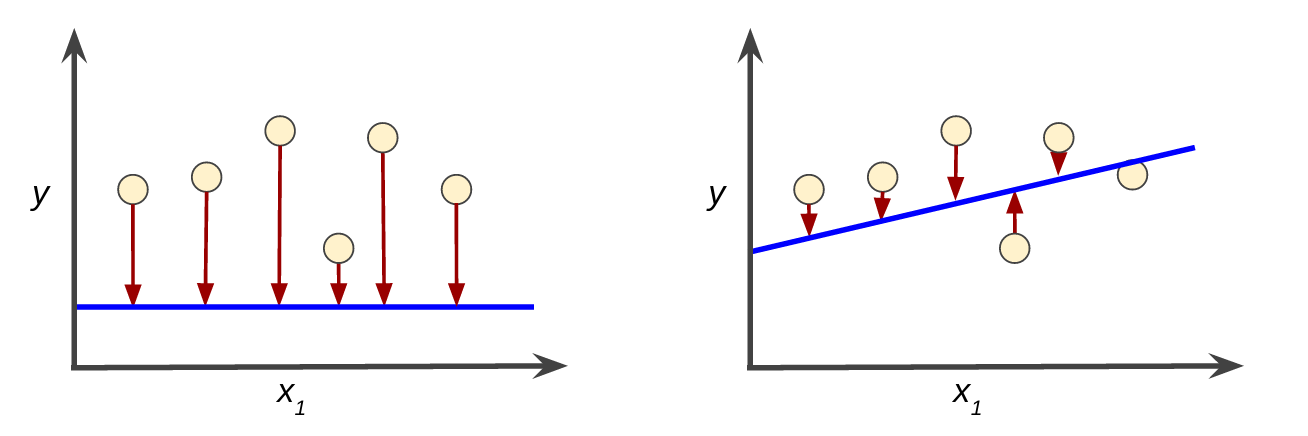
\includegraphics[width=\textwidth]{images/LossSideBySide.png}
\end{frame}

%%%

\begin{frame}{Training and Loss}
\begin{itemize}
\item Notice that the arrows in the left plot are much longer than their counterparts in the right plot. 

\medskip    
\item Clearly, the right blue line is a much better predictive model than the left blue line.

\medskip
\item The linear regression models we examine here use a loss function called {\bf squared loss} (also known as $L_2$ loss). 
\end{itemize}
\end{frame}

%%%

\begin{frame}{Training and Loss}
\begin{itemize}
\item Let $w=(b,w_1,\ldots,w_n)$ the parameters of the model (its weights and bias).

\item Consider a labeled example with features $x=(x_1,\ldots,x_n)$ and label $y$.

\item The model predicts

$$ \hat{y} = f_w(x) = b + \sum_{j=1}^n w_j x_j$$

\item The squared loss for a single example the difference between the label (observation) $y$ and the prediction $\hat{y}$:

$$ (y - \hat{y})^2 $$    
\end{itemize}
\end{frame}

%%%

\begin{frame}{Training and Loss}
\begin{itemize}
\item {\bf Mean square error (MSE)} is the average squared loss per example over the whole dataset
    
$$ \mathrm{MSE}(w) = \frac{1}{m} \sum_{i=1}^m (y^{(i)} - \hat{y}^{(i)})^2 $$

\medskip
\item $m$ is the number of examples.

\medskip
\item $x^{(i)}=(x^{(i)}_1,\ldots,x^{(i)}_n)$ and $y^{(i)}$ are the features and the label of the $i$th example.

\medskip
\item $\hat{y}^{(i)}$ is the prediction of the model. More formally, 
$$ \hat{y} = f_w(x^{(i)}) = b + \sum_{j=1}^n w_j x^{(i)}_j $$
\end{itemize}
\end{frame}

%%%

\begin{frame}{Training and Loss}
\begin{itemize}
    \item Although MSE is commonly-used in machine learning, it is neither the only practical loss function nor the best loss function for all circumstances.
\end{itemize}
\end{frame}

%%%

\begin{frame}{Key Terms}
\begin{itemize}
\item empirical risk minimization
\item loss
\item mean squared error
\item squared loss
\item training
\end{itemize}
\end{frame}

\end{document}